
\subsection{Introduction to the Problem}
\emph{Gray Codes} are enumerations of objects in a set such that there is 
minimal amount change to transition from $Obj_{i}$ to $Obj_{i+1}$. In order 
to define the mininmal amount of change, a basic operation needs to be defined that constitutes a change
from one object to the next. For example, enumerating all binary strings of length $N$ defines the basic 
operation as flipping a bit. The better the Gray Code, the lower the number of 
bit flips are required to transition from $BinaryString_{i}$ to $BinaryString_{i+1}$. 
The problem of finding a Gray Code for generating canonical ladders from $OptL\{\pi\}$ is inspired by finding the most efficient way to produce a 
single ladder acting as a  representative for all $OptL\{\pi_{N}\}$. The formal statement of the problem is the following; given a value 
$N\geq3$ where $N \in Z$, generate a canonical ladder from $OptL\{\pi_{N}\}$ for each $\pi$ of order $N$.
For example, let $N=4$, then there are twenty-four, or $N!$ permutations 
of order $N$. These permutations, listed lexicographically (smallest to largest)
are:

\begin{center}
\small{1234 1243}\newline
\small{1324 1342}\newline
\small{1423 1432}\newline
\small{2134 2143}\newline
\small{2314 2341}\newline
\small{2413 2431}\newline
\small{3124 3142}\newline
\small{3214 3241}\newline
\small{3412 3421}\newline
\small{4123 4132}\newline
\small{4213 4231}\newline
\small{4312 4321}\newline
\end{center}
Each of these permutations has zero or more ladders in each of their respective 
$OptL\{\pi\}$. The Gray Code problem asks, what is the most efficient way to enumerate 
a canonical ladder from each $OptL\{\pi_{i}\}$ such that a minimal change from 
one canonical ladder can be applied to said ladder resulting in the canonical 
ladder in $OptL\{\pi_{i+1}\}$. In this thesis, four Gray Codes were used to generate the canonical 
ladders for each $OptL\{\pi_{N}\}$. Each of these Gray Codes are modifications of already existing 
Gray Codes for generating all permutations of order $N$. The Gray Codes used 
are Steinhaus-Jonson-Trotter Gray Code, the Zaks Gray Code, Heaps Gray Code and lexicographic Gray Code.
Unlike with most Gray Codes, there are two basic operations defined for 
the modified Gray Codes for enumerating canonical ladders from $OptL\{\pi\}$.
The first basic operation is the insertion or deletion of a bar. The second 
operation is the swap of two bars. 

\begin{theorem} The first basic operation 
is necessary to transition from $L_{i}$ to $L_{i+1}$ whereas the second operation is not.
\end{theorem}

\begin{proof}
    Suppose that the first of the two basic operations was not necessary.
    Let $L_{i}$ be the canonical representative of $OptL\{\pi_{i}\}$ of 
    order $N$. Let $L_{i+1}$ be the canonical representative of $OptL\{\pi_{i+1}\}$
    of order $N$. Let $x$ be any labelled bar in $L_{i}$. Note that $x$ represents an 
    inversion in $\pi_{i}$. If $x$ is not removed from $L_{i+1}$ then $L_{i+1}$ 
    must have an additional bar, otherwise $\pi_{i}$ and $\pi_{i+1}$ are the same permutation.
    Thus, at least one new bar, $y$ is inserted to $L_{i+1}$. Suppose that $x$ is removed $L_{i+1}$,
    then a removal operation has been performed in order to transition from $L_{i}$ 
    to $L_{i+1}$. In both cases the first basic operation is performed. If neither of the above 
    cases are true, then $L_{i}=L_{i+1}$ which is a contradiction.
\end{proof}
\begin{proof}
    Suppose that the second basic operation is necessary. Consider the ladder 
    for the idendity permutation of order $N$. Let $L_{Id}$ denote this ladder. 
    Seeing as it is the only ladder in $OptL\{\pi_{Id}\}$ then it must be the 
    canonical representative. Let $L_{i+1}$ be the canonical representative of 
    the next permutation's $OptL\{\pi\}$. Seeing as $L_{Id}$ has no bars to swap, 
   then it is impossible to derive $L_{i+1}$ from $L_{Id}$ by performing a 
   swap operation. Thus, it is not necessary to permform a swap operation to transition 
   from a canonical representative to the next representative. In fact, in the above example 
   it is impossible to perform a swap operation. 
\end{proof}
The canonical representative was chosen in two ways. The first way of 
chosing the canonical representative was to always choose the root ladder from each $OptL\{\pi_{N}\}$.
The rationale for always choosing the root ladder was due to the fact that every 
permutation has a root ladder in its $OptL\{\pi\}$ whereas not every permutation 
has a non-root ladder. For example, given the permutation $(2,1,4,3)$, $OptL\{(2,1,4,3)\}$
has only one ladder which is the root ladder. This is because there are only two 
bars in the ladder, thus there is no swap operation that can be performed.
\begin{theorem}
    If $|OptL\{\pi\}|=1$ then the ladder is the root ladder.
\end{theorem} 
\begin{proof}
    The root ladder is defined as the ladder whose clean level is one.
    This means either there is no bar of a lesser element above the route a 
    greater element. Keeping in mind that the clean level of the root ladder is one, next consider what is meant by a  \emph{child bar}
     which is a bar to the bottom left or right of a given bar $x$. Within the context of the root ladder, 
     if the left endpoint of the child bar is directly below the right end point of $x$ then the child is a 
    right child of $x$. If the right end point of the child bar is directly 
    below the left end point of $x$ then it is a left child. 
    Keeping in mind the root ladder has not undergone any right swap operations, then
    if a child is a right child 
    then the child belongs to the same route of $x$ in the root ladder. 
    Let $R_{m}$ denote this route. Let $x$ be a bar representing an inversion with element $m$ and $k$.
    The right child of $x$ is a bar which represents an inversion 
    with $m$ and some element to the right of $k$. Suppose this was not the case, 
    then this would mean that the right child of $x$ was either a bar representing an inversion 
    between some element $m'$ that was greater than $m$ or lesser than $m$. If $m'$ was 
    greater than $m$ then this would be a contradiction seeing as $x$ would be above the bar of a route 
    of a greater element which contradicts the definition of the root ladder. On the other hand if 
    $m'$ were lesser than $m$, then $m$ would form an inversion with $m'$ and therefore 
    the bar representing this inversion would be part of the route of $m$ route. Thus, the right child 
    of a bar $x$ belongs to the same route as $x$ in the root ladder.\par The left child of $x$
    represents an inversion with some lesser element than $m$ and $k$. Suppose this was not the case, 
    then the left child could belong to a route greater than $m$, but if that were the case, this contradicts 
    the definition of the root ladder.
    Thus the first element of the left child must belong to the route of some lesser element than $m$. Next suppose that 
    the lesser element of the left child of $x$ was not $k$. Let this element be termed $k'$.
    $k'$ forms an inversion with the greater element of the left child of $x$. But since the greater element of the left child is less than $m$, 
    then $m$ would also form an inversion with $k'$. Thus, the bar of $m$ and $k'$ would be the parent of the left child, which is also 
    a contradiction, seeing as the left child is the child of bar $x$. Therefore the left child of $x$ must be a bar that 
    it belongs to the route of a lesser element than $m$ and its lesser element is $k$.\par 
    Please refer to FIG--- to view an example of a root ladder with left and right children.\pagebreak

    
\end{proof}


\begin{figure}[!htp]
    \begin{center}
    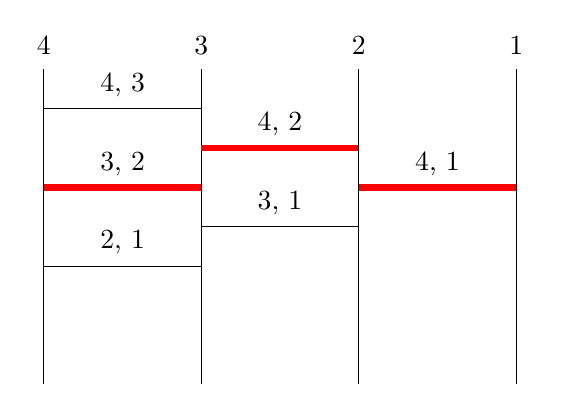
\begin{tikzpicture}
        \draw(0, 0) to (0, 4);
            \node at(0, 4.3){4};
             \draw(0, 3.5) to (2, 3.5);
                \node at(1, 3.8){4, 3};
            
            \draw[line width=0.8mm, red](0, 2.5) to (2, 2.5);
                \node at(1, 2.8){3, 2};

            \draw(0, 1.5) to (2, 1.5);
                \node at(1, 1.8){2, 1};
        \draw(2, 0) to (2, 4);
            \node at(2, 4.3){3};
                \draw[line width=.8mm, red](2, 3) to (4, 3);
                    \node at(3, 3.3){4, 2};
           
                \draw(2, 2) to (4, 2);
                    \node at(3, 2.3){3, 1};
        \draw(4, 0) to (4, 4);
             \node at(4, 4.3){2};
                \draw[line width=0.8mm, red](4, 2.5) to (6, 2.5);
                    \node at (5, 2.8){4, 1};
        \draw(6, 0) to (6, 4);
            \node at(6, 4.3){1};


    \end{tikzpicture}
    \end{center}
    \caption{The root ladder of $(4,3,2,1)$. Note that bar 4,2 is the parent of bar 3,2 and 4,1. Also note that 
    bar 3, 2 is the the left child of 4, 2 and 4, 1 is the right child.}
\end{figure}

The second way to choose the canonical representative is to use a greedy algorithm 
in order to choose the best representative from the next $OptL\{\pi_{N}\}$. 
The is based on comparing the canonical representative from $OptL\{\pi_{i}\}$ with all the ladders in
$OptL\{\pi_{i+1}\}$and choosing the ladder from $OptL\{\pi_{i+1}\}$ that had the least number of 
changes from the canonical ladder from $OptL\{\pi_{i}\}$. Each Gray Code provides a different representative.
Both of the basic operations are used in order to determine the optimal canonical representative.
The canonical representative from $OptL\{\pi_{i+1}\}$ is the ladder with the least number of insertions/deletions 
and least number of swaps when compared to the canonical representative from $OptL\{\pi_{i}\}$.
The canonical representative for $OptL\{\pi_{1}\}$ is the root ladder for the idendity permutation.\par 
In order to see a comparision for the two canonical representative selection methods for permutations of 
size 3 using the modified Zaks algorithm please refer to figure --\pagebreak

\begin{figure}[!htp]
   
 \begin{minipage}{0.1\textwidth}
    \begin{flushleft}
    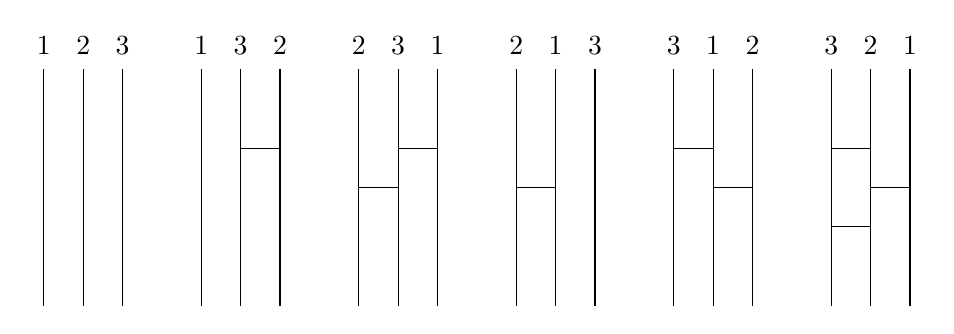
\begin{tikzpicture}

        %%l1
        \draw(0, 0) to (0, 3);
            \node at (0, 3.3){1};
        \draw(0.5, 0) to (0.5, 3);
            \node at (0.5, 3.3){2};
        \draw(1, 0) to (1, 3);
            \node at(1, 3.3){3};

            %%\draw(2.2, 1.5) to (2.8, 1.5);
        %%L2
           \draw(2, 0) to (2, 3);
            \node at (2, 3.3){1};
        \draw(2.5, 0) to (2.5, 3);
            \node at (2.5, 3.3){3};
                \draw(2.5, 2) to (3, 2);
        \draw(3, 0) to (3, 3);
            \node at(3, 3.3){2};

        %%L3
            \draw(4, 0) to (4, 3);
                \node at(4, 3.3){2};
                \draw(4, 1.5) to (4.5, 1.5);
            \draw(4.5, 0) to (4.5, 3);
                \node at(4.5, 3.3){3};
                \draw(4.5, 2) to (5, 2);
            \draw(5, 0) to (5, 3);
                \node at(5, 3.3){1};
        %%L4
            \draw(6, 0) to (6, 3);
                \node at(6, 3.3){2};
                \draw(6, 1.5) to (6.5, 1.5);
            \draw(6.5, 0) to (6.5, 3);
                \node at(6.5, 3.3){1};
            \draw(7, 0) to (7, 3);
                \node at(7, 3.3){3};

         %%L5
            \draw(8, 0) to (8, 3);
                \node at(8, 3.3){3};
                \draw(8, 2) to (8.5, 2);
            \draw(8.5, 0) to (8.5, 3);
                \node at(8.5, 3.3){1};
                \draw(8.5, 1.5) to (9, 1.5);
            \draw(9, 0) to (9, 3);
                \node at(9, 3.3){2};

         %%L6
            \draw(10, 0) to (10, 3);
                \node at(10, 3.3){3};
                \draw(10, 2) to (10.5, 2);
                \draw(10, 1) to (10.5, 1);
            \draw(10.5, 0) to (10.5, 3);
                \node at(10.5, 3.3){2};
                \draw(10.5, 1.5) to (11, 1.5);
            \draw(11, 0) to (11, 3);
                \node at(11, 3.3){1};
    \end{tikzpicture}
\end{flushleft}
\end{minipage}
 

\begin{minipage}{0.1\textwidth}
    \begin{flushleft}
    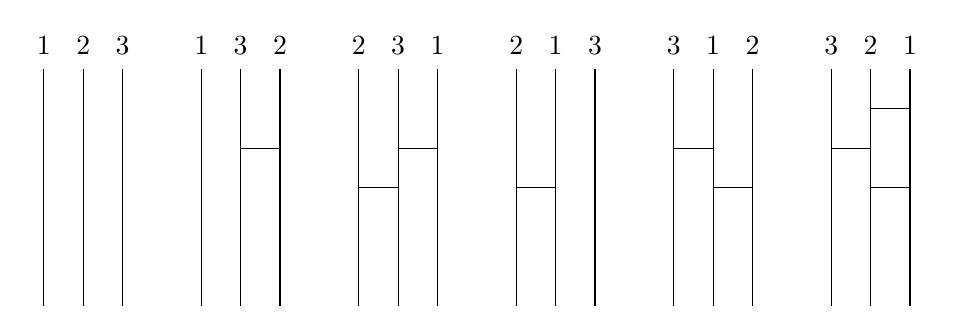
\begin{tikzpicture}

        %%l1
        \draw(0, 0) to (0, 3);
            \node at (0, 3.3){1};
        \draw(0.5, 0) to (0.5, 3);
            \node at (0.5, 3.3){2};
        \draw(1, 0) to (1, 3);
            \node at(1, 3.3){3};

            %%\draw(2.2, 1.5) to (2.8, 1.5);
        %%L2
           \draw(2, 0) to (2, 3);
            \node at (2, 3.3){1};
        \draw(2.5, 0) to (2.5, 3);
            \node at (2.5, 3.3){3};
                \draw(2.5, 2) to (3, 2);
        \draw(3, 0) to (3, 3);
            \node at(3, 3.3){2};

        %%L3
            \draw(4, 0) to (4, 3);
                \node at(4, 3.3){2};
                \draw(4, 1.5) to (4.5, 1.5);
            \draw(4.5, 0) to (4.5, 3);
                \node at(4.5, 3.3){3};
                \draw(4.5, 2) to (5, 2);
            \draw(5, 0) to (5, 3);
                \node at(5, 3.3){1};
        %%L4
            \draw(6, 0) to (6, 3);
                \node at(6, 3.3){2};
                \draw(6, 1.5) to (6.5, 1.5);
            \draw(6.5, 0) to (6.5, 3);
                \node at(6.5, 3.3){1};
            \draw(7, 0) to (7, 3);
                \node at(7, 3.3){3};

         %%L5
            \draw(8, 0) to (8, 3);
                \node at(8, 3.3){3};
                \draw(8, 2) to (8.5, 2);
            \draw(8.5, 0) to (8.5, 3);
                \node at(8.5, 3.3){1};
                \draw(8.5, 1.5) to (9, 1.5);
            \draw(9, 0) to (9, 3);
                \node at(9, 3.3){2};

         %%L6
            \draw(10, 0) to (10, 3);
                \node at(10, 3.3){3};
                \draw(10, 2) to (10.5, 2);
                
            \draw(10.5, 0) to (10.5, 3);
                \node at(10.5, 3.3){2};
                \draw(10.5, 1.5) to (11, 1.5);
                \draw(10.5, 2.5) to (11, 2.5);
            \draw(11, 0) to (11, 3);
                \node at(11, 3.3){1};
    \end{tikzpicture}
\end{flushleft}
\end{minipage}
\caption{The canonical representatives from $N=3$ for all $OptL\{\pi_{3}\}$
using the modified Zaks Gray Code. The top row represents the root ladder as the canonical ladder.
The bottom row represents the greedy choice for the canonical ladder. Notice how the last ladder in the rows 
differ from each other.}
\end{figure}



    
